%%%%%%%%%%%%%%%%%%%%%%%%%%%%%%%%%%%%%%%%%%%%%%%%%%%%%%%%%%%%%%%%%%%%%%%%
% Plantilla TFG/TFM
% Universidad de Murcia. Facultad de Informática
% Realizado por: José Manuel Requena Plens
% Modificado: Pablo José Rocamora Zamora
% Contacto: pablojoserocamora@gmail.com
%%%%%%%%%%%%%%%%%%%%%%%%%%%%%%%%%%%%%%%%%%%%%%%%%%%%%%%%%%%%%%%%%%%%%%%%

\chapter{Estado del Arte}
\label{cap:estado_arte}

Para comprender la arquitectura y las decisiones de diseño adoptadas en este Trabajo de Fin de Grado, es necesario establecer una base teórica sobre las tecnologías subyacentes. Este capítulo revisa los conceptos clave en los que se apoya el sistema desarrollado: la Web Semántica, los Modelos de Lenguaje de Gran Escala (LLMs) y los paradigmas emergentes de Inteligencia Artificial como la Generación Aumentada por Recuperación (RAG) y los agentes autónomos.

\section{Web Semántica y Grafos de Conocimiento}

La Web Semántica, propuesta originalmente por Tim Berners-Lee en 2001 \cite{berners2001semantic}, busca extender la web actual dotando a la información de un significado bien definido, permitiendo que ordenadores y personas trabajen en cooperación. A diferencia de la web tradicional, basada en documentos vinculados mediante hipertexto, la Web Semántica se fundamenta en la publicación de datos estructurados que pueden ser comprendidos y procesados automáticamente por las máquinas.

El núcleo de esta visión son los Grafos de Conocimiento (\textit{Knowledge Graphs}), estructuras de datos que representan entidades del mundo real y sus interrelaciones de forma explícita y rica en semántica \cite{hogan2021knowledge}. Estas estructuras permiten no solo almacenar hechos aislados, sino también inferir nuevo conocimiento a partir del existente mediante la aplicación de reglas lógicas y ontologías, que definen las clases y propiedades del dominio modelado. En el contexto de este trabajo, los Grafos de Conocimiento han cobrado una gran relevancia para la integración de datos y la resolución de consultas complejas de manera estructurada.

\subsection{Resource Description Framework (RDF)}
RDF es el estándar principal para modelar información en la Web Semántica \cite{w3c_rdf}. La información se estructura en forma de tripletas que representan una relación entre dos entidades, por lo que el modelo de datos está estructurado en forma de grafo, donde cada nodo es una entidad y cada arista es una relación entre dos entidades: \textit{Sujeto}, \textit{Predicado} y \textit{Objeto}. 

Estas tripletas pueden serializarse en distintos formatos, siendo \textit{nt} (N-Triples) uno de los más eficientes para el almacenamiento, tiempo de procesamiento y consultas complejas que requieran pasar de unas entidades a otras (multi-hop queries), como se muestra en la siguiente figura.


\begin{figure}[h]
    \centering
    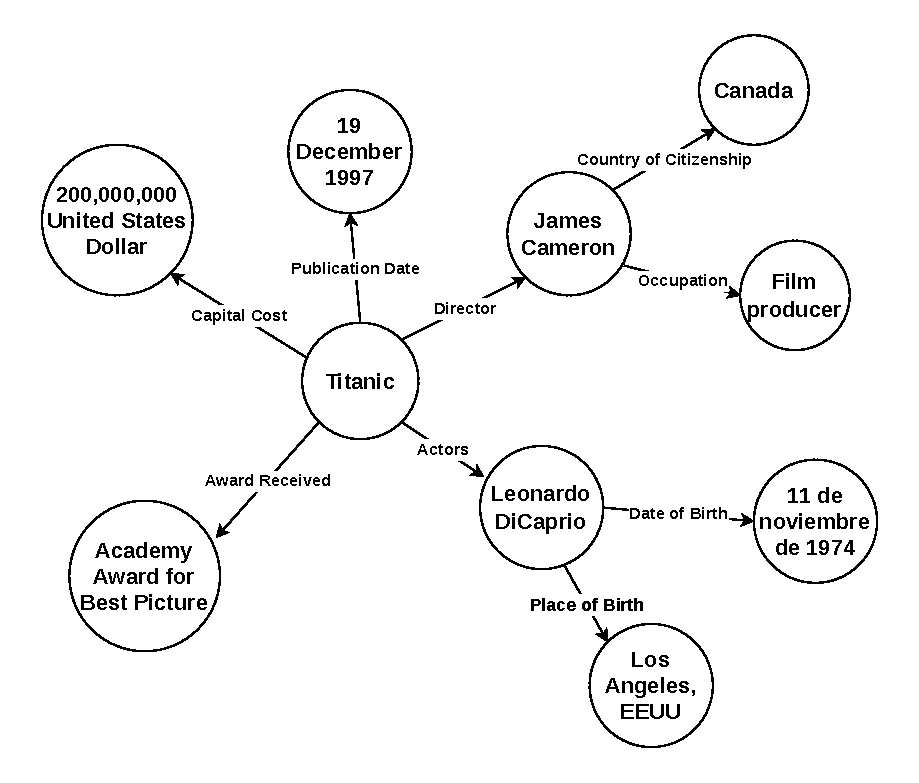
\includegraphics[width=0.8\textwidth]{archivos/Grafo_Conocimiento.pdf}
    \caption{Ejemplo de grafo de conocimiento sobre el dominio del cine.}
    \label{fig:grafo_conocimiento}
\end{figure}

\subsection{SPARQL}
SPARQL (\textit{SPARQL Protocol and RDF Query Language}) es el lenguaje de consulta estándar para bases de datos RDF \cite{w3c_sparql}. Permite realizar consultas complejas sobre grafos, filtrar resultados y explorar las relaciones semánticas entre entidades. Aunque es extremadamente potente y preciso, su curva de aprendizaje es muy pronunciada, lo que justifica la necesidad de construir interfaces en lenguaje natural para democratizar el acceso a los datos, como se propone en este TFG.

\subsection{Wikidata}
Wikidata es una base de conocimiento libre, colaborativa y multilingüe que actúa como almacenamiento central para los datos estructurados de sus proyectos hermanos, como Wikipedia \cite{vrandecic2014wikidata}. Dado su enorme volumen de datos y su estructura semántica abierta y en constante evolución, Wikidata se ha consolidado como una de las fuentes de conocimiento general más importantes del mundo, sirviendo como origen de los datos sobre la industria del cine extraídos para este proyecto.

\section{Modelos de Lenguaje de Gran Escala (LLMs)}

Los Modelos de Lenguaje de Gran Escala (LLMs) son sistemas de Inteligencia Artificial compuestos por redes neuronales masivas, fundamentadas principalmente en la arquitectura \textit{Transformer} \cite{vaswani2017attention}. Estos modelos son preentrenados sobre volúmenes ingentes de texto utilizando aprendizaje autosupervisado, lo que les dota de capacidades sin precedentes en tareas de comprensión, síntesis, traducción y generación de lenguaje natural \cite{zhao2023survey}.

En el ecosistema actual de los LLMs, podemos distinguir diversas familias y enfoques, diferenciados principalmente por su apertura, arquitectura y el tipo de entrenamiento recibido:

\begin{itemize}
    \item \textbf{Modelos Propietarios y Comerciales (e.g., GPT-4, Gemini, Claude):} Esta categoría incluye modelos desarrollados por empresas privadas, cuyo código fuente y pesos no son públicos y se acceden generalmente a través de una API. La familia GPT (\textit{Generative Pre-trained Transformer}) de OpenAI \cite{openai2023gpt4} destaca por su rendimiento puntero en razonamiento y generación de código. Paralelamente, modelos como Gemini de Google \cite{geminoteam2023gemini} introducen capacidades multimodales nativas desde su diseño base, mientras que Claude de Anthropic \cite{anthropic2023claude} se enfoca en la seguridad y en el procesamiento de enormes ventanas de contexto.
    \item \textbf{Modelos Abiertos (e.g., LLaMA, Mistral):} En contraposición, la comunidad de código abierto ha impulsado modelos cuyos pesos están disponibles para investigación e implementación local. La familia LLaMA (\textit{Large Language Model Meta AI}) \cite{touvron2023llama} es uno de sus máximos exponentes, demostrando que es posible alcanzar un rendimiento competitivo con modelos propietarios utilizando menos parámetros pero entrenados sobre conjuntos de datos más grandes y de mayor calidad. Esto reduce los costes de inferencia y permite su ejecución en infraestructuras locales.
\end{itemize}

Las diferencias fundamentales entre modelos cerrados (como GPT) y abiertos (como LLaMA) residen en la accesibilidad, la privacidad y el control de los datos. Mientras GPT-4 ofrece el estado del arte a expensas de enviar datos a servidores externos, LLaMA y otros modelos de peso abierto permiten desplegar soluciones totalmente privadas (\textit{on-premise}), un aspecto crítico y alineado con los requisitos no funcionales de este Trabajo de Fin de Grado.

Sin embargo, en el contexto de la recuperación de información real y precisa, los LLMs presentan dos limitaciones críticas inherentes a su naturaleza estocástica:
\begin{enumerate}
    \item \textbf{Conocimiento estático:} El modelo solo conoce la información disponible hasta el momento de su entrenamiento, requiriendo reentrenamientos costosos para actualizarse.
    \item \textbf{Alucinaciones:} Tendencia a generar respuestas altamente plausibles a nivel sintáctico pero incorrectas cuando el modelo no dispone de la información requerida en sus pesos internos.
\end{enumerate}

Para mitigar estos problemas, especialmente en aplicaciones de dominio específico, es estrictamente necesario acoplar el LLM con fuentes de conocimiento externas fidedignas.

\section{Generación Aumentada por Recuperación (RAG)}

La Generación Aumentada por Recuperación (\textit{Retrieval-Augmented Generation}, RAG) es una arquitectura \cite{lewis2020retrieval} que mejora sustancialmente la fiabilidad de las respuestas de un LLM al integrar un sistema de recuperación de información y al obligar al LLM a basar sus respuestas en la información específica proporcionada en el momento de la consulta. En un flujo RAG estándar:
\begin{enumerate}
    \item El usuario realiza una pregunta en lenguaje natural.
    \item El sistema busca información relevante en una base de datos externa.
    \item La información recuperada se inyecta en el \textit{prompt} (contexto) del LLM.
    \item El LLM formula la respuesta final basándose en el contexto documentado proporcionado, en lugar de depender únicamente de su memoria interna.
\end{enumerate}

En este TFG, se aplica una variante más estructurada de RAG, a menudo referida como \textbf{Graph RAG} o \textbf{Text-to-SPARQL RAG}. En lugar de recuperar fragmentos de texto mediante similitud vectorial (que puede ser imprecisa), el modelo se encarga de generar el código lógico (SPARQL) necesario para interrogar un Grafo de Conocimiento de forma determinista, garantizando respuestas estructuradas y exactas.

\section{Agentes Autónomos y LangChain}

Un paso más allá del uso estático de LLMs es el paradigma de la Inteligencia Artificial Agéntica. Un agente de IA es un sistema que utiliza un LLM como su "motor de razonamiento" central para decidir dinámicamente qué acciones tomar, qué herramientas utilizar y en qué orden.

A diferencia de un flujo de código secuencial clásico, un agente puede observar el resultado de una acción y reaccionar. Por ejemplo, si el agente genera una consulta SPARQL que, al ejecutarse en el motor de base de datos, devuelve un error de sintaxis, el agente puede leer dicho error, reflexionar sobre el fallo, autocorregir el código y volver a intentar la consulta. Este bucle de retroalimentación dota al sistema de una robustez crítica frente a la variabilidad de las respuestas del modelo.

\textbf{LangChain} \cite{langchain} es el \textit{framework} de desarrollo de código abierto líder en el ecosistema para la creación de aplicaciones impulsadas por modelos de lenguaje. Proporciona las abstracciones necesarias para construir cadenas de procesamiento complejas, integrar herramientas externas, gestionar la memoria de las conversaciones y orquestar el flujo cognitivo de agentes autónomos orientados a la recuperación de conocimiento estructurado.

\section{Aplicaciones similares de consulta con LLMs y Repositorios Semánticos}

El uso de LLMs para interrogar bases de datos estructuradas ha experimentado un gran avance. Históricamente, el acceso a repositorios semánticos requería el dominio de lenguajes formales como SPARQL, lo que suponía una barrera de entrada importante para usuarios sin un profundo perfil técnico.

Con el auge de la IA Generativa, han surgido diversas aproximaciones para la tarea de \textit{Text-to-SPARQL} o de consulta de bases de datos mediante lenguaje natural \cite{yin2024text}. Entre las soluciones más destacables se encuentran:

\begin{itemize}
    \item \textbf{Sistemas Text-to-SQL y herramientas de Chat sobre BD:} Aunque en un principio han estado orientadas a bases de datos relacionales, herramientas como Chat2DB o los agentes SQL integrados en LangChain han sentado las bases metodológicas. Estos sistemas inyectan el esquema de la base de datos en el contexto del LLM para que interprete la estructura y genere sentencias ejecutables válidas de consulta.
    \item \textbf{KGQA (\textit{Knowledge Graph Question Answering}):} Son arquitecturas específicamente diseñadas para interactuar con grafos de conocimiento. Las aproximaciones recientes combinan la recuperación semántica con técnicas de LLMs, utilizando herramientas de desambiguación de entidades previas para localizar correctamente los nodos iniciales dentro del grafo.
    \item \textbf{Frameworks Híbridos (e.g. OntoGPT):} Proyectos de investigación e industria que exploran un ciclo de vida completo: emplean LLMs tanto para extraer información no estructurada e insertarla en repositorios semánticos, como para posteriormente explotar dichos repositorios facilitando consultas conversacionales ricas.
\end{itemize}

A diferencia de las interfaces \textit{Text-to-SPARQL} estáticas de traducción única (donde la inferencia inicial dicta el éxito o fracaso de la consulta), la propuesta tecnológica de este TFG apuesta por la \textbf{resiliencia} a través de agentes autónomos. La integración de un bucle de retroalimentación o reflexión en la propia consulta permite corregir fallos sintácticos de forma dinámica antes de trasladar el resultado al usuario, reduciendo el impacto de las alucinaciones del modelo.